
A mother lets me watch her kids and says to me: Show the children a game. When she returns, she sees me teaching them to gamble with
dice. She angrily exclaims I didn't mean that sort of game! Must the exclusion
of the game with dice have come before his mind when he gave me the order?

It's true that she did mean not that sort of game. but she need not have had the conscious thought at the time of the request. Somehow her request made a normative division of proper responses.

If you find this puzzling that, nonetheless, what you did was an inappropriate response to her request, then you are trapped in a possibly Cartesian trap. You're missing what distinguishes a sign from a piece of wood.

From: \cite{wittgenstein2010philosophical}

Frac $\frac{a}{b}$!

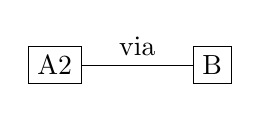
\begin{tikzpicture}
  \path (0,0) node[draw] (A) {A2};
  \path (2,0) node[draw] (B) {B};
  \draw (A) -- (B) node[midway,above = 0 em] {via};
\end{tikzpicture}


\begin{tikzpicture}[node distance=1cm, auto,]
    %nodes
    \node[punkt] (market) {Market (b)};
    \node[punkt, inner sep=5pt,below=0.5cm of market]
    (formidler) {Intermediaries (c)};
    % We make a dummy figure to make everything look nice.
    \node[above=of market] (dummy) {};
    \node[right=of dummy] (t) {Ultimate borrower}
      edge[pil,bend left=45] (market.east) % edges are used to connect two nodes
      edge[pil, bend left=45] (formidler.east); % .east since we want
                                                % consistent style
    \node[left=of dummy] (g) {Ultimate lender}
      edge[pil, bend right=45] (market.west)
      edge[pil, bend right=45] (formidler.west)
      edge[pil,<->, bend left=45] node[auto] {Direct (a)} (t);
   \end{tikzpicture}

   \vspace{1em}
   \emph{Inspired by figure 1.1 in ``Financial Markets and Institutions'' 5E
     by Howells and Bain.}


